\Level 0 {Random numbers}
\label{sec:stl:random}

The \ac{STL} has a
\indextermbus{random number}{generator}
that is more general and more flexible than the C~version (section~\ref{sec:crand}),
discussed below.

\begin{itemize}
\item There are several generators that give uniformly distributed
  numbers;
\item then there are distributions that translate this to non-uniform
  or discrete distributions.
\end{itemize}

First you declare an engine; later this will be transformed into a distribution:
\begin{lstlisting}
std::default_random_engine generator;
\end{lstlisting}

This generator will start at the same value everytime.
You can seed it:
\begin{lstlisting}
std::random_device r;
std::default_random_engine generator{ r() };
\end{lstlisting}

\Level 1 {Distributions}

The most common mode of generating random number
is to pick them from a distribution.
For instance, a uniform distribution between given bounds:
\begin{lstlisting}
std::uniform_real_distribution<float> distribution(0.,1.);
\end{lstlisting}
A roll of the dice would result from:
\begin{lstlisting}
std::uniform_int_distribution<int> distribution(1,6);
\end{lstlisting}

\begin{slide}{Random generators and distributions}
  \label{sl:std-rand-device}
  \begin{itemize}
  \item Random device
\begin{lstlisting}
std::default_random_engine generator;
% random seed:
std::random_device r;
std::default_random_engine generator{ r() };
\end{lstlisting}

\item Distributions:
\begin{lstlisting}
std::uniform_real_distribution<float> distribution(0.,1.);
std::uniform_int_distribution<int> distribution(1,6);
\end{lstlisting}

\item Sample from the distribution:
\begin{lstlisting}
std::default_random_engine generator;
std::uniform_int_distribution<> distribution(0,nbuckets-1);
random_number = distribution(generator);
\end{lstlisting}

  \item Do not use the old C-style \indexc{random}!
  \end{itemize}
\end{slide}

\begin{block}{Random floats}
  \label{sl:stl:rand}
  \verbatimsnippet{c11rand}
\end{block}

\begin{block}{Dice throw}
  \label{sl:stl:rand16}
\begin{lstlisting}
// set the default generator
std::default_random_engine generator;

// distribution: ints 1..6
std::uniform_int_distribution<int> distribution(1,6);

// apply distribution to generator:
int dice_roll = distribution(generator);
  // generates number in the range 1..6 
\end{lstlisting}
\end{block}

\begin{block}{Poisson distribution}
  \label{sl:st:poisson}
  Another distribution is the \indextermbus{Poisson}{distribution}:
\begin{lstlisting}
std::default_random_engine generator;
float mean = 3.5;
std::poisson_distribution<int> distribution(mean);
int number = distribution(generator);
\end{lstlisting}
\end{block}

You might be tempted not include not only the invocation of a \ac{RNG}
in a routine that needs it,
but also the definition.
This is not going to work, because the generator will be initialized
every time you call the function.
You can fix this by making the generator variable \indexc{static}.

\begin{block}{Global engine}
  \label{sl:static-random}
  Wrong approach:
  \snippetwithoutput{nonrandomint}{rand}{nonrandom}
  Good approach:
  \snippetwithoutput{truerandomint}{rand}{truerandom}
\end{block}

\begin{exercise}
  Chapter~\ref{ch:walk} has a case study of using random numbers
  for simulating a \indextermbus{random}{walk}.
\end{exercise}

\begin{comment}
  \Level 1 {Exercise}

  A \indextermbus{random}{walk} is a process
  where a position gets updated every time step.
  Every update is a displacement over a unit distance,
  in some random direction:
  \[ p_{i+1} = p_i + \overrightarrow r, \qquad \left|r\right|=1. \]

  This was originally invented as a way of modeling the spread of mosquitos:
  if a mosquito flies the same distance every day, but in a random direction,
  how far can it reach in its life span.

  \begin{exercise}
    Make \lstinline{Mosquito} class with a \lstinline{step} method.
    Calling this method updates the position of the mosquito
    by a random unit distance.
    Make the class so that the location can be in any number of dimensions.

    The main problem here is to compute the random displacement.
    \begin{itemize}
    \item You can use trigoniometric functions to compute a point on the unit sphere.
    \item You also generate a point in a unit cube, and project it on the unit sphere.
    \end{itemize}
    In both cases, you have to be careful to let the points be uniform.
  \end{exercise}

  When you're convinced that your code is correct, explore the mathematics:

  \begin{exercise}
    Explore how far a mosquito can get from its starting point in $N$ days.
    Does this depend on the dimensionality~$d$?

    You may need to repeat every experiment a number of times
    to make it statistically significant.
  \end{exercise}
\end{comment}

\Level 1 {Permutations}

The function \indexc{shuffle} shuffles an array.
Coupled with the \indexc{iota} function this easily gives a permutation:

\verbatimsnippet{vectorshuffle}

\Level 1 {C random function}
\label{sec:crand}

There is an easy (but not terribly great)
\indextermbus{random number}{generator}
that works the same as in~C.
%
\begin{lstlisting}
#include <random>
using std::rand;
float random_fraction =
    (float)rand()/(float)RAND_MAX;
\end{lstlisting}
%
The function \indexc{rand} yields an \lstinline{int}
--~a different one every time you call it~--
in the range from zero to \indexc{RAND_MAX}.
Using scaling and casting you can then produce a fraction between zero
and one with the above code.

This generator has some problems.

\begin{itemize}
\item The C random number generator has a period of~$2^{15}$, which may be small.
\item There is only one generator algorithm, which is implementation-dependent,
  and has no guarantees on its quality.
\item There are no mechanisms fort ransforming the sequence to a range.
  The common idiom
\begin{lstlisting}
int under100 = rand() % 100
\end{lstlisting}
is biased to small numbers. Figure~\ref{fig:rand7mod3} shows this
for a generator with period~7 taken modulo~3.
\end{itemize}

\begin{figure}[t]
  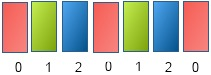
\includegraphics{rand7mod3}
  \caption{Low number bias of a random number generator taken module}
  \label{fig:rand7mod3}
\end{figure}

If you run your program twice, you will twice get the same sequence of
random numbers. That is great for debugging your program but not if
you were hoping to do some statistical analysis. Therefore you can set
the \indextermbus{random number}{seed} from which the random sequence
starts by the \indexc{srand} function. Example:
\begin{lstlisting}
srand(time(NULL));
\end{lstlisting}
seeds the random number generator from the current time.
This call should happen only once, typically somewhere high up in your main.

